\section{Results}
The evaluation of the model happened in three stages. The first part completely relied on simulation results. The second was the physical simulation of separate modules independently on the breadboard. Finally, the complete prototype was built and tested.
\par
The requirements that needed to be met, and the method utilized to test whether they have been met are as follows:

\begin{figure}[h]
    \resizebox{\columnwidth}{!}{
        \begin{tabular}{|c|c|c|}
            \toprule
            Design              & \multirow{2}{*}{Target Value} & \multirow{2}{*}{Testing Method}          \\
            Requirement         &                               &                                          \\
            \midrule\midrule
            Spectrum            & Specified Amplitude Ratios    & \multirow{3}{*}{Stimulation}             \\
            \cmidrule(lr){1-2}
            Wave pattern        & Exponential-Decay             &                                          \\
            \cmidrule(lr){1-2}
            Power Efficiency    & 75\%                          &                                          \\
            \midrule
            Speakers            & 4$\Omega$-16$\Omega$ \& 1W-5W & Prototype                                \\
            \midrule
            Quality \& Loudness & 40dB-75dB                     & \multirow{2}{*}{Stimulation/ Prototype } \\
            \cmidrule(lr){1-2}
            Datasheet           & parameters                    &                                          \\
            \bottomrule
        \end{tabular}}
\end{figure}
\subsection{Simulation}
\subsubsection*{Wave Generator}
The outputs of oscillators are very stable although a slight variation in the frequencies($\pm 3$) was observed. The following figures illustrate the observed decay pattern and stable waveform from an oscillator.
\begin{figure}[h]
    \begin{subfigure}{.48\columnwidth}
        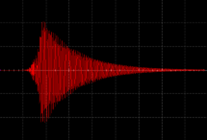
\includegraphics[width=.8\columnwidth]{wave_sim}
        \caption*{Envelope Pattern}
    \end{subfigure}
    \begin{subfigure}{.48\columnwidth}
        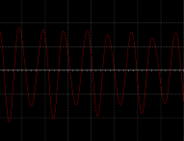
\includegraphics[width=\columnwidth]{s_wave_sim}
        \caption*{Wave Pattern}
    \end{subfigure}
\end{figure}

The output of the scalar adder looked similar to the original waveform and the spectrums were closely matched. Somehow at the simulation stage, sound outputs failed to match. Expected and observed wave characteristics as follows:
\begin{figure}[h]
    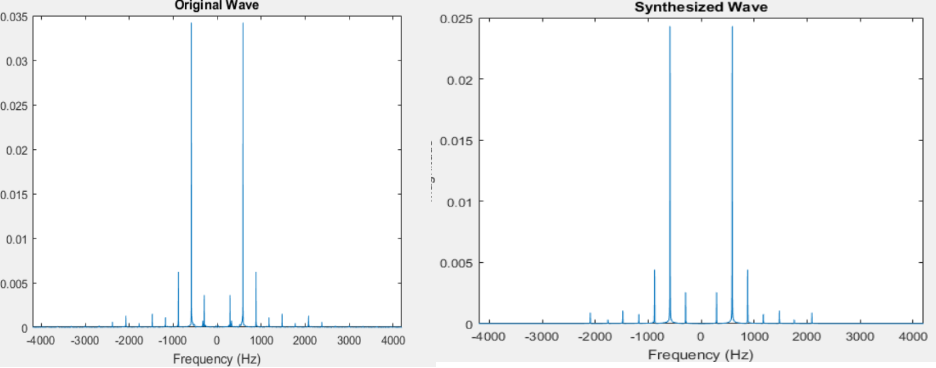
\includegraphics[width=\columnwidth]{spectrum}
\end{figure}
\\
These stages are operated at low power and the oscillations are normally in a damped state. This allows keeping the overall output of the wave generator to be in a normally-off state which is crucial for power efficiency.
\subsubsection*{Amplifier}
Although the wave synthesis process is limited to frequencies lower than 5kHz, it is initially planned to implement an amplifier that has a constant gain throughout the full audible range(up to 20kHz). From the observations, the model was limited to 12kHz which is expected due to imperfections in transistor behaviors.
\begin{figure}[h]
    \begin{subfigure}{.48\columnwidth}
        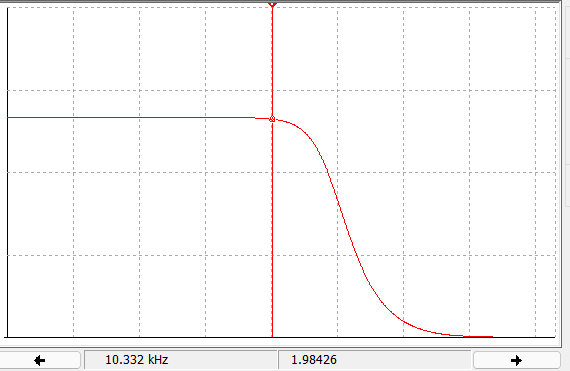
\includegraphics[width=.8\columnwidth]{magnitude}
        \caption*{Voltage Gain}
    \end{subfigure}
    \begin{subfigure}{.48\columnwidth}
        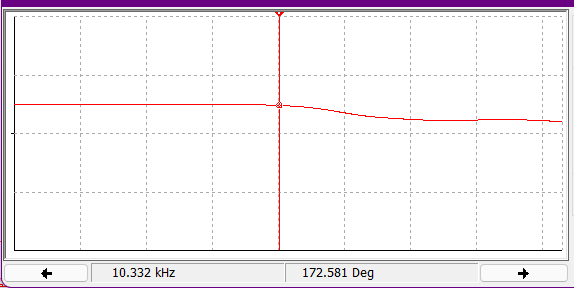
\includegraphics[width=\columnwidth]{phase}
        \caption*{Phase}
    \end{subfigure}
\end{figure}
\\
From the simulation, it was confirmed that the feedback resistance gives linear control over the gain of the amplifier.
\begin{enumerate}
    \item \textbf{Input Resistance} : \textbf{28.2k$\Omega$}\\The input resistance was determined by using the multimeter tool to measure the current drawn from the source and dividing the source voltage by the measured value.
    \item \textbf{Output Impedance} : \textbf{1.9$\Omega$}\\The output impedance was calculated by using voltmeter tool and constant current source. The input was sort-circuited and constant current source applied in the output. Then the voltmeter reading in the current source was measured.
          $$R_{out}=\frac{V_{read}}{I_{source}}$$
    \item \textbf{Bandwidth} : \textbf{200Hz-12kHz}\\Bandwidth was determined using the bode-plot of the amplifier. The region where gain stays constant is only considered.
    \item \textbf{Gain}(8$\Omega$) : \textbf{50dB-70dB}\\The gain was determined using the wattmeter tool between the input source and speaker input.
    \item \textbf{Power Efficiency} : \textbf{69\%}\\
          $$\eta=\frac{P_L}{P_S}\times 100\%$$
    \item \textbf{Safety Measurements :} \\
          The maximum current path was observed to conduct 600mA in the worst case. This was considered in the maximum power calculations and component selections.
\end{enumerate}

\subsection{Circuit Blocks}
\subsubsection*{Wave Generator}
Noise-free stable wave pattern is observed at each oscillator. The measured frequencies vary in the range of 10Hz as expected due to the imperfection in resistance selection. Although the wave pattern observed had  clipping effect it was observed that they could be eliminated by fine-tuning.
\begin{figure}[h]
    \begin{subfigure}{.48\columnwidth}
        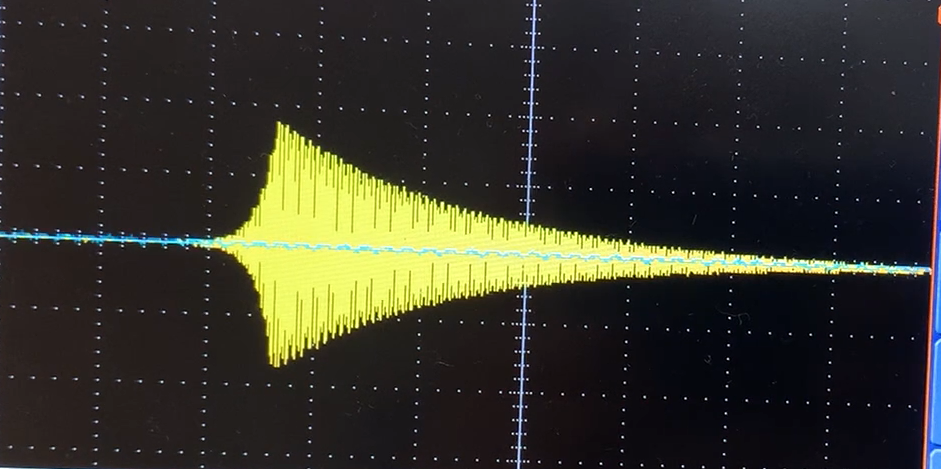
\includegraphics[width=.9\columnwidth]{wein_phy_2}
        \caption*{Envelope Pattern}
    \end{subfigure}
    \begin{subfigure}{.48\columnwidth}
        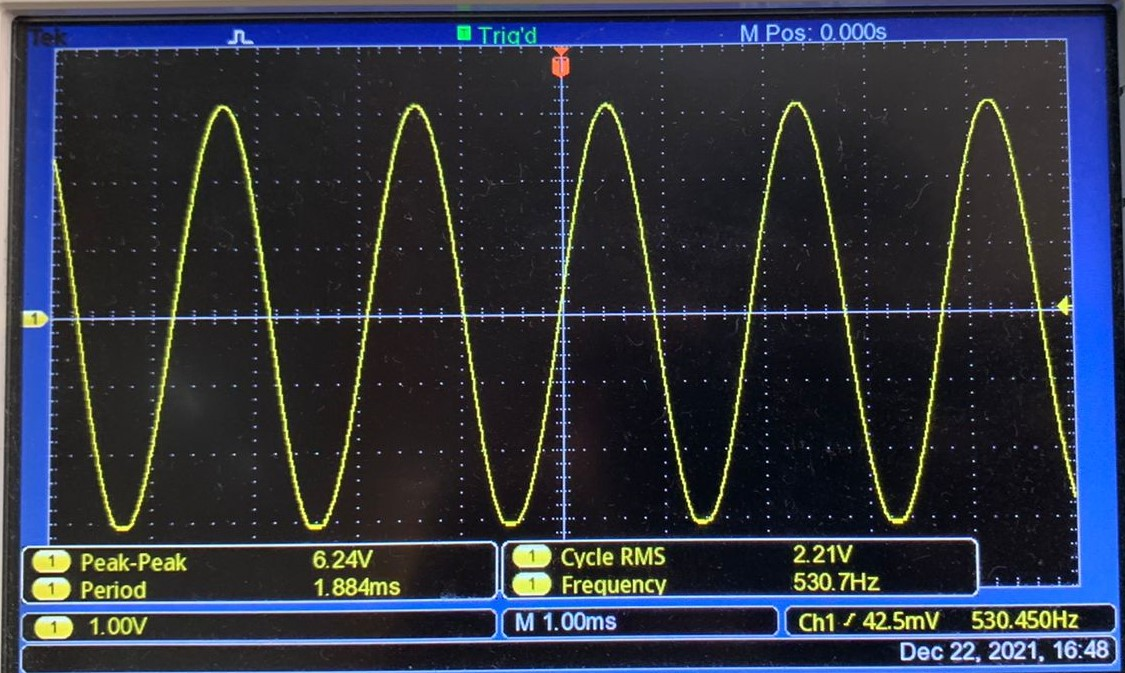
\includegraphics[width=.8\columnwidth]{wein_phy}
        \caption*{Wave Pattern}
    \end{subfigure}
\end{figure}

\subsubsection*{Amplifier}
The parameters measured were varied with simulation results.
\begin{enumerate}
    \item \textbf{Input Resistance} : \textbf{43M$\Omega$}\\The input impedance was determined by using a digital multimeter to measure the current being drawn from the input for an audio input of 0.1mA (peak to peak), with the output open-circuited.
    \item \textbf{Output Impedance} : \textbf{10$\Omega$}\\Output impedance was measured using the voltmeter, from the open circuit reading in the output terminal ($V_O$) and the reading in the 8$\Omega$ load ($V_L$).
          $$R_{out}=R_L\times\frac{V_L}{V_O}$$
    \item \textbf{Bandwidth} : \textbf{200Hz-12kHz}\\Bandwidth was determined using bode-plot of the amplifier. The region where gain stays constant was only considered.
    \item \textbf{Power Efficiency} : \textbf{63\%}\\
          Efficiency was determined by inspecting the supply and speaker inputs.
    \item \textbf{Maximum Current} : \textbf{0.4A}
\end{enumerate}
The performance of the amplifier with song output from a mobile phone is also inspected at this stage. The results are as follows.
\begin{figure}[h]
    \centering
    \includegraphics[width=.75\columnwidth]{song}
    \caption*{\textbf{Song Wave} : Input - Yellow \& Output - Blue}
\end{figure}

\subsection{Integrated-Circuit}
The wave generator is cascaded with the amplifier to create the final prototype of the design. The sound output of the completed circuit was observed very familiarly with the c-wave of the piano. The waveforms of the original wave and finely tuned wave output are as follows:
\begin{figure}[h]
    \begin{subfigure}{.48\columnwidth}
    \centering
    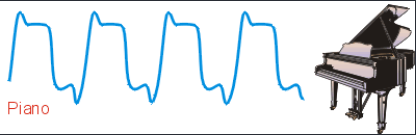
\includegraphics[width=\columnwidth]{c_expect}
    \caption*{Original Wave}
    \end{subfigure}
    \begin{subfigure}{.48\columnwidth}
        \centering
        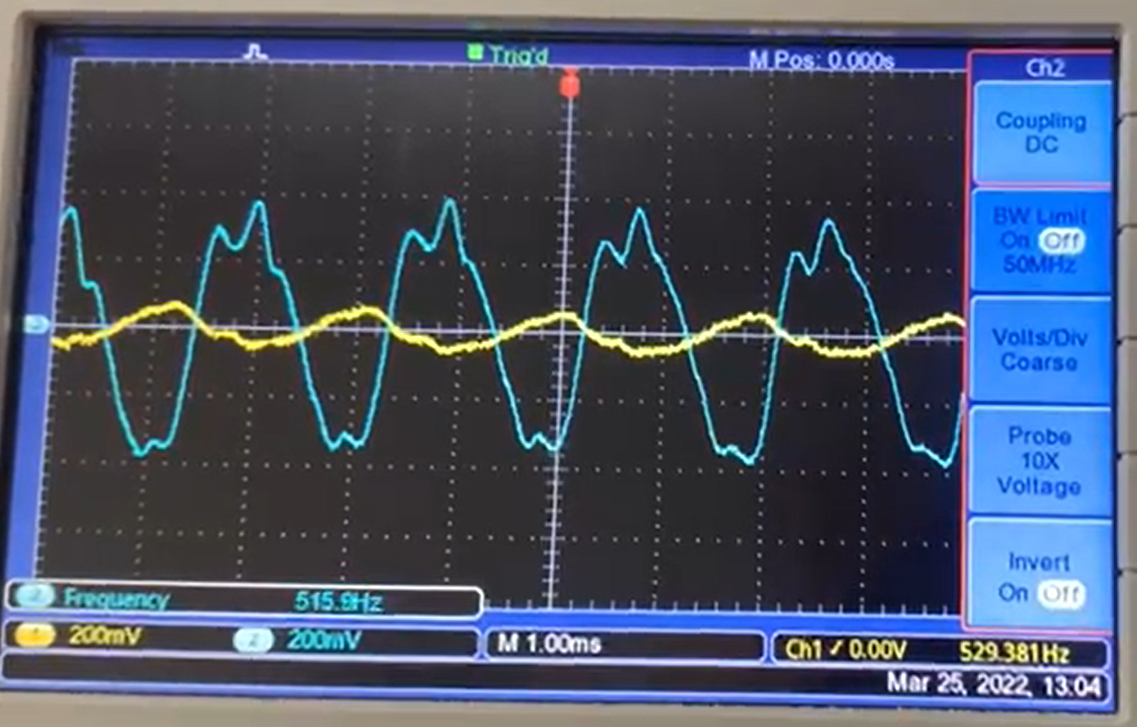
\includegraphics[width=.7\columnwidth]{o_wave_o}
        \caption*{Tuned Output}
    \end{subfigure}
    \newline
    \begin{subfigure}{.48\columnwidth}
        \centering
    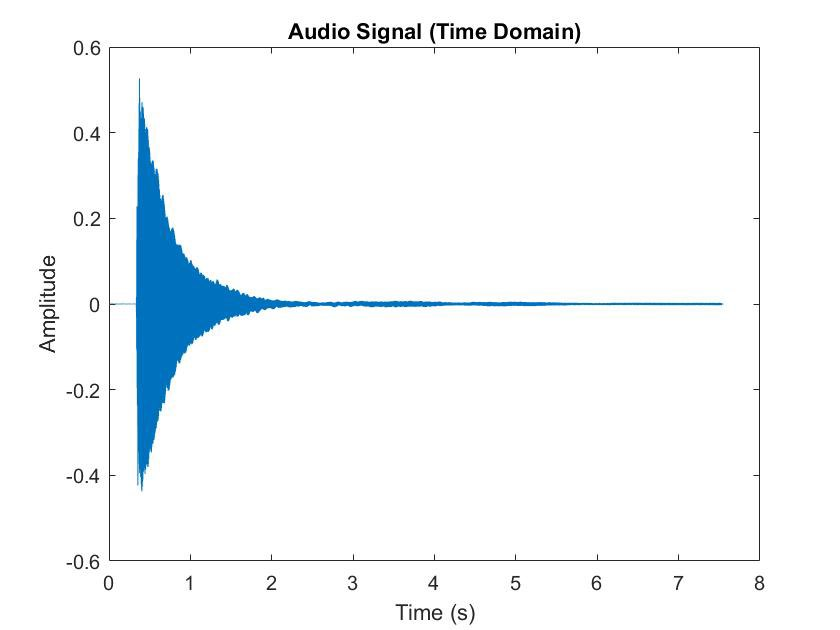
\includegraphics[width=.75\columnwidth]{final_wave_expectation}
    \caption*{Original Envelope}
\end{subfigure}
\begin{subfigure}{.48\columnwidth}
    \centering
    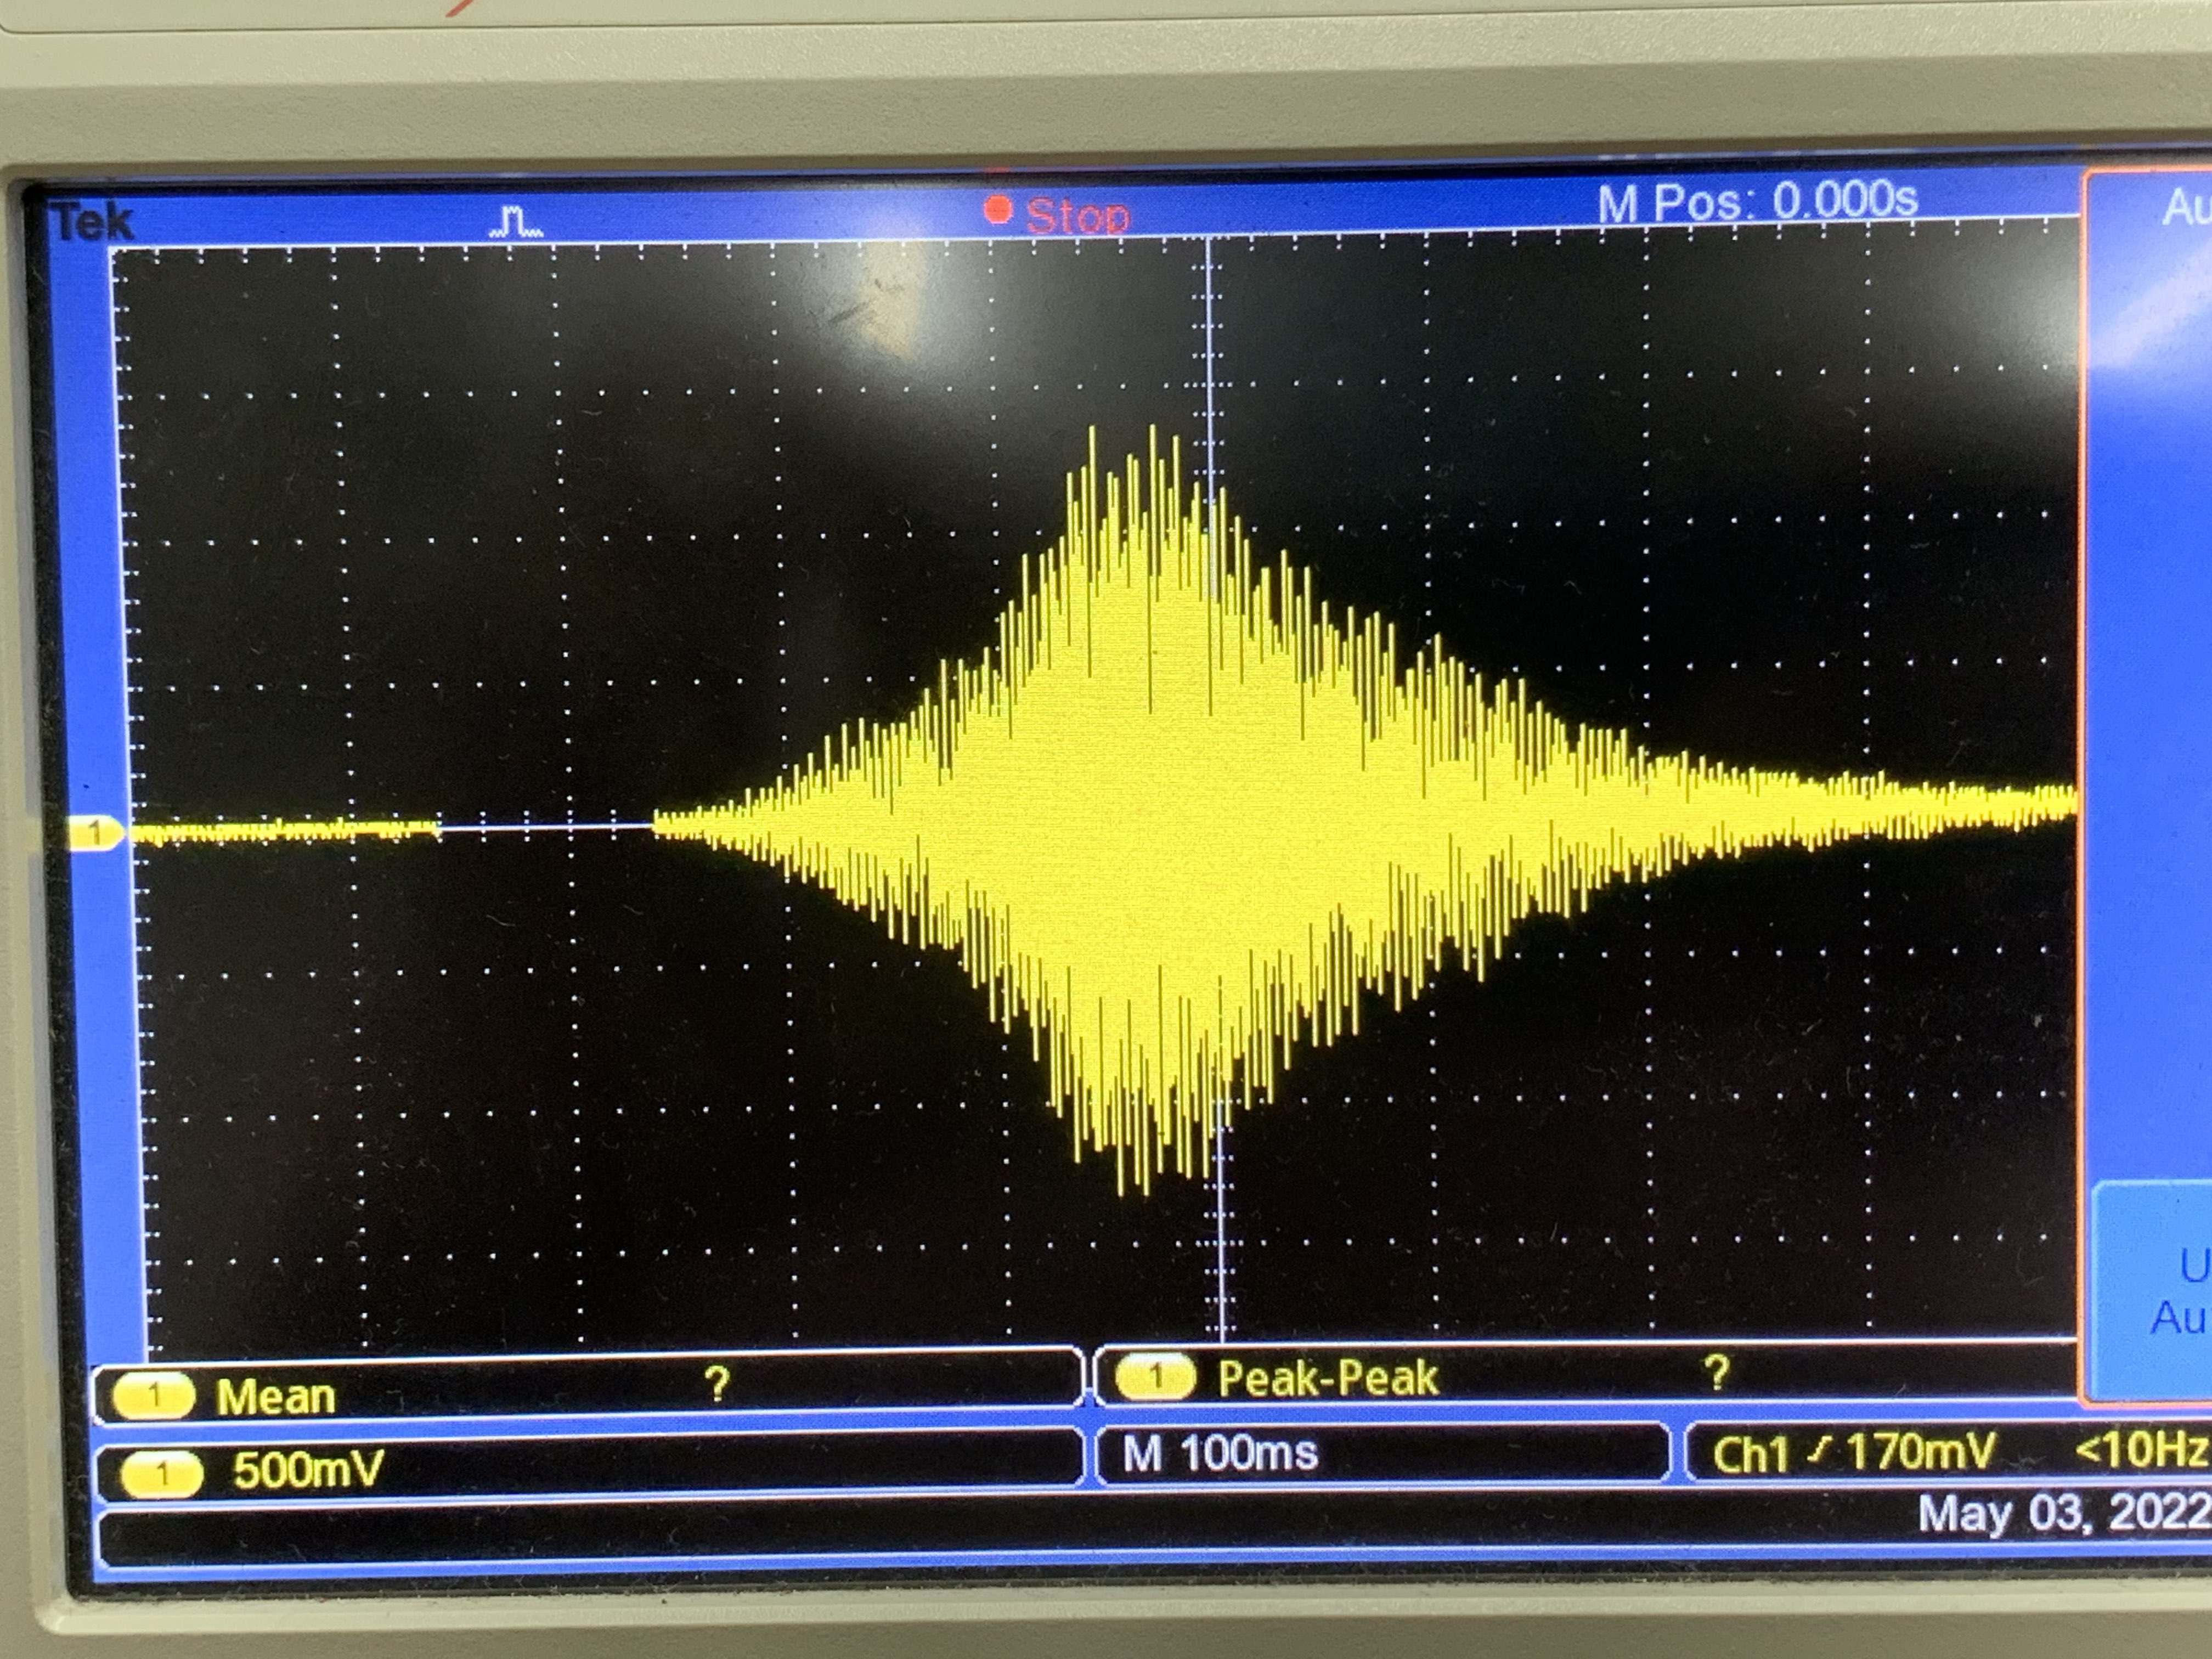
\includegraphics[width=.75\columnwidth]{final_wave}
    \caption*{Observation}
\end{subfigure}
\end{figure}
\\
Although a small elongation was observed at the start of oscillation this could also be controlled by parallel resistance that is responsible for the start of the oscillation. We suspected this behavior is due to an increase in impedance imposed by tracks.